
% Default to the notebook output style

    


% Inherit from the specified cell style.




    
\documentclass[11pt]{article}

    
    
    \usepackage[T1]{fontenc}
    % Nicer default font (+ math font) than Computer Modern for most use cases
    \usepackage{mathpazo}

    % Basic figure setup, for now with no caption control since it's done
    % automatically by Pandoc (which extracts ![](path) syntax from Markdown).
    \usepackage{graphicx}
    % We will generate all images so they have a width \maxwidth. This means
    % that they will get their normal width if they fit onto the page, but
    % are scaled down if they would overflow the margins.
    \makeatletter
    \def\maxwidth{\ifdim\Gin@nat@width>\linewidth\linewidth
    \else\Gin@nat@width\fi}
    \makeatother
    \let\Oldincludegraphics\includegraphics
    % Set max figure width to be 80% of text width, for now hardcoded.
    \renewcommand{\includegraphics}[1]{\Oldincludegraphics[width=.8\maxwidth]{#1}}
    % Ensure that by default, figures have no caption (until we provide a
    % proper Figure object with a Caption API and a way to capture that
    % in the conversion process - todo).
    \usepackage{caption}
    \DeclareCaptionLabelFormat{nolabel}{}
    \captionsetup{labelformat=nolabel}

    \usepackage{adjustbox} % Used to constrain images to a maximum size 
    \usepackage{xcolor} % Allow colors to be defined
    \usepackage{enumerate} % Needed for markdown enumerations to work
    \usepackage{geometry} % Used to adjust the document margins
    \usepackage{amsmath} % Equations
    \usepackage{amssymb} % Equations
    \usepackage{textcomp} % defines textquotesingle
    % Hack from http://tex.stackexchange.com/a/47451/13684:
    \AtBeginDocument{%
        \def\PYZsq{\textquotesingle}% Upright quotes in Pygmentized code
    }
    \usepackage{upquote} % Upright quotes for verbatim code
    \usepackage{eurosym} % defines \euro
    \usepackage[mathletters]{ucs} % Extended unicode (utf-8) support
    \usepackage[utf8x]{inputenc} % Allow utf-8 characters in the tex document
    \usepackage{fancyvrb} % verbatim replacement that allows latex
    \usepackage{grffile} % extends the file name processing of package graphics 
                         % to support a larger range 
    % The hyperref package gives us a pdf with properly built
    % internal navigation ('pdf bookmarks' for the table of contents,
    % internal cross-reference links, web links for URLs, etc.)
    \usepackage{hyperref}
    \usepackage{longtable} % longtable support required by pandoc >1.10
    \usepackage{booktabs}  % table support for pandoc > 1.12.2
    \usepackage[inline]{enumitem} % IRkernel/repr support (it uses the enumerate* environment)
    \usepackage[normalem]{ulem} % ulem is needed to support strikethroughs (\sout)
                                % normalem makes italics be italics, not underlines
    

    
    
    % Colors for the hyperref package
    \definecolor{urlcolor}{rgb}{0,.145,.698}
    \definecolor{linkcolor}{rgb}{.71,0.21,0.01}
    \definecolor{citecolor}{rgb}{.12,.54,.11}

    % ANSI colors
    \definecolor{ansi-black}{HTML}{3E424D}
    \definecolor{ansi-black-intense}{HTML}{282C36}
    \definecolor{ansi-red}{HTML}{E75C58}
    \definecolor{ansi-red-intense}{HTML}{B22B31}
    \definecolor{ansi-green}{HTML}{00A250}
    \definecolor{ansi-green-intense}{HTML}{007427}
    \definecolor{ansi-yellow}{HTML}{DDB62B}
    \definecolor{ansi-yellow-intense}{HTML}{B27D12}
    \definecolor{ansi-blue}{HTML}{208FFB}
    \definecolor{ansi-blue-intense}{HTML}{0065CA}
    \definecolor{ansi-magenta}{HTML}{D160C4}
    \definecolor{ansi-magenta-intense}{HTML}{A03196}
    \definecolor{ansi-cyan}{HTML}{60C6C8}
    \definecolor{ansi-cyan-intense}{HTML}{258F8F}
    \definecolor{ansi-white}{HTML}{C5C1B4}
    \definecolor{ansi-white-intense}{HTML}{A1A6B2}

    % commands and environments needed by pandoc snippets
    % extracted from the output of `pandoc -s`
    \providecommand{\tightlist}{%
      \setlength{\itemsep}{0pt}\setlength{\parskip}{0pt}}
    \DefineVerbatimEnvironment{Highlighting}{Verbatim}{commandchars=\\\{\}}
    % Add ',fontsize=\small' for more characters per line
    \newenvironment{Shaded}{}{}
    \newcommand{\KeywordTok}[1]{\textcolor[rgb]{0.00,0.44,0.13}{\textbf{{#1}}}}
    \newcommand{\DataTypeTok}[1]{\textcolor[rgb]{0.56,0.13,0.00}{{#1}}}
    \newcommand{\DecValTok}[1]{\textcolor[rgb]{0.25,0.63,0.44}{{#1}}}
    \newcommand{\BaseNTok}[1]{\textcolor[rgb]{0.25,0.63,0.44}{{#1}}}
    \newcommand{\FloatTok}[1]{\textcolor[rgb]{0.25,0.63,0.44}{{#1}}}
    \newcommand{\CharTok}[1]{\textcolor[rgb]{0.25,0.44,0.63}{{#1}}}
    \newcommand{\StringTok}[1]{\textcolor[rgb]{0.25,0.44,0.63}{{#1}}}
    \newcommand{\CommentTok}[1]{\textcolor[rgb]{0.38,0.63,0.69}{\textit{{#1}}}}
    \newcommand{\OtherTok}[1]{\textcolor[rgb]{0.00,0.44,0.13}{{#1}}}
    \newcommand{\AlertTok}[1]{\textcolor[rgb]{1.00,0.00,0.00}{\textbf{{#1}}}}
    \newcommand{\FunctionTok}[1]{\textcolor[rgb]{0.02,0.16,0.49}{{#1}}}
    \newcommand{\RegionMarkerTok}[1]{{#1}}
    \newcommand{\ErrorTok}[1]{\textcolor[rgb]{1.00,0.00,0.00}{\textbf{{#1}}}}
    \newcommand{\NormalTok}[1]{{#1}}
    
    % Additional commands for more recent versions of Pandoc
    \newcommand{\ConstantTok}[1]{\textcolor[rgb]{0.53,0.00,0.00}{{#1}}}
    \newcommand{\SpecialCharTok}[1]{\textcolor[rgb]{0.25,0.44,0.63}{{#1}}}
    \newcommand{\VerbatimStringTok}[1]{\textcolor[rgb]{0.25,0.44,0.63}{{#1}}}
    \newcommand{\SpecialStringTok}[1]{\textcolor[rgb]{0.73,0.40,0.53}{{#1}}}
    \newcommand{\ImportTok}[1]{{#1}}
    \newcommand{\DocumentationTok}[1]{\textcolor[rgb]{0.73,0.13,0.13}{\textit{{#1}}}}
    \newcommand{\AnnotationTok}[1]{\textcolor[rgb]{0.38,0.63,0.69}{\textbf{\textit{{#1}}}}}
    \newcommand{\CommentVarTok}[1]{\textcolor[rgb]{0.38,0.63,0.69}{\textbf{\textit{{#1}}}}}
    \newcommand{\VariableTok}[1]{\textcolor[rgb]{0.10,0.09,0.49}{{#1}}}
    \newcommand{\ControlFlowTok}[1]{\textcolor[rgb]{0.00,0.44,0.13}{\textbf{{#1}}}}
    \newcommand{\OperatorTok}[1]{\textcolor[rgb]{0.40,0.40,0.40}{{#1}}}
    \newcommand{\BuiltInTok}[1]{{#1}}
    \newcommand{\ExtensionTok}[1]{{#1}}
    \newcommand{\PreprocessorTok}[1]{\textcolor[rgb]{0.74,0.48,0.00}{{#1}}}
    \newcommand{\AttributeTok}[1]{\textcolor[rgb]{0.49,0.56,0.16}{{#1}}}
    \newcommand{\InformationTok}[1]{\textcolor[rgb]{0.38,0.63,0.69}{\textbf{\textit{{#1}}}}}
    \newcommand{\WarningTok}[1]{\textcolor[rgb]{0.38,0.63,0.69}{\textbf{\textit{{#1}}}}}
    
    
    % Define a nice break command that doesn't care if a line doesn't already
    % exist.
    \def\br{\hspace*{\fill} \\* }
    % Math Jax compatability definitions
    \def\gt{>}
    \def\lt{<}
    % Document parameters
    \title{1301150434\_IF3910}
    
    
    

    % Pygments definitions
    
\makeatletter
\def\PY@reset{\let\PY@it=\relax \let\PY@bf=\relax%
    \let\PY@ul=\relax \let\PY@tc=\relax%
    \let\PY@bc=\relax \let\PY@ff=\relax}
\def\PY@tok#1{\csname PY@tok@#1\endcsname}
\def\PY@toks#1+{\ifx\relax#1\empty\else%
    \PY@tok{#1}\expandafter\PY@toks\fi}
\def\PY@do#1{\PY@bc{\PY@tc{\PY@ul{%
    \PY@it{\PY@bf{\PY@ff{#1}}}}}}}
\def\PY#1#2{\PY@reset\PY@toks#1+\relax+\PY@do{#2}}

\expandafter\def\csname PY@tok@w\endcsname{\def\PY@tc##1{\textcolor[rgb]{0.73,0.73,0.73}{##1}}}
\expandafter\def\csname PY@tok@c\endcsname{\let\PY@it=\textit\def\PY@tc##1{\textcolor[rgb]{0.25,0.50,0.50}{##1}}}
\expandafter\def\csname PY@tok@cp\endcsname{\def\PY@tc##1{\textcolor[rgb]{0.74,0.48,0.00}{##1}}}
\expandafter\def\csname PY@tok@k\endcsname{\let\PY@bf=\textbf\def\PY@tc##1{\textcolor[rgb]{0.00,0.50,0.00}{##1}}}
\expandafter\def\csname PY@tok@kp\endcsname{\def\PY@tc##1{\textcolor[rgb]{0.00,0.50,0.00}{##1}}}
\expandafter\def\csname PY@tok@kt\endcsname{\def\PY@tc##1{\textcolor[rgb]{0.69,0.00,0.25}{##1}}}
\expandafter\def\csname PY@tok@o\endcsname{\def\PY@tc##1{\textcolor[rgb]{0.40,0.40,0.40}{##1}}}
\expandafter\def\csname PY@tok@ow\endcsname{\let\PY@bf=\textbf\def\PY@tc##1{\textcolor[rgb]{0.67,0.13,1.00}{##1}}}
\expandafter\def\csname PY@tok@nb\endcsname{\def\PY@tc##1{\textcolor[rgb]{0.00,0.50,0.00}{##1}}}
\expandafter\def\csname PY@tok@nf\endcsname{\def\PY@tc##1{\textcolor[rgb]{0.00,0.00,1.00}{##1}}}
\expandafter\def\csname PY@tok@nc\endcsname{\let\PY@bf=\textbf\def\PY@tc##1{\textcolor[rgb]{0.00,0.00,1.00}{##1}}}
\expandafter\def\csname PY@tok@nn\endcsname{\let\PY@bf=\textbf\def\PY@tc##1{\textcolor[rgb]{0.00,0.00,1.00}{##1}}}
\expandafter\def\csname PY@tok@ne\endcsname{\let\PY@bf=\textbf\def\PY@tc##1{\textcolor[rgb]{0.82,0.25,0.23}{##1}}}
\expandafter\def\csname PY@tok@nv\endcsname{\def\PY@tc##1{\textcolor[rgb]{0.10,0.09,0.49}{##1}}}
\expandafter\def\csname PY@tok@no\endcsname{\def\PY@tc##1{\textcolor[rgb]{0.53,0.00,0.00}{##1}}}
\expandafter\def\csname PY@tok@nl\endcsname{\def\PY@tc##1{\textcolor[rgb]{0.63,0.63,0.00}{##1}}}
\expandafter\def\csname PY@tok@ni\endcsname{\let\PY@bf=\textbf\def\PY@tc##1{\textcolor[rgb]{0.60,0.60,0.60}{##1}}}
\expandafter\def\csname PY@tok@na\endcsname{\def\PY@tc##1{\textcolor[rgb]{0.49,0.56,0.16}{##1}}}
\expandafter\def\csname PY@tok@nt\endcsname{\let\PY@bf=\textbf\def\PY@tc##1{\textcolor[rgb]{0.00,0.50,0.00}{##1}}}
\expandafter\def\csname PY@tok@nd\endcsname{\def\PY@tc##1{\textcolor[rgb]{0.67,0.13,1.00}{##1}}}
\expandafter\def\csname PY@tok@s\endcsname{\def\PY@tc##1{\textcolor[rgb]{0.73,0.13,0.13}{##1}}}
\expandafter\def\csname PY@tok@sd\endcsname{\let\PY@it=\textit\def\PY@tc##1{\textcolor[rgb]{0.73,0.13,0.13}{##1}}}
\expandafter\def\csname PY@tok@si\endcsname{\let\PY@bf=\textbf\def\PY@tc##1{\textcolor[rgb]{0.73,0.40,0.53}{##1}}}
\expandafter\def\csname PY@tok@se\endcsname{\let\PY@bf=\textbf\def\PY@tc##1{\textcolor[rgb]{0.73,0.40,0.13}{##1}}}
\expandafter\def\csname PY@tok@sr\endcsname{\def\PY@tc##1{\textcolor[rgb]{0.73,0.40,0.53}{##1}}}
\expandafter\def\csname PY@tok@ss\endcsname{\def\PY@tc##1{\textcolor[rgb]{0.10,0.09,0.49}{##1}}}
\expandafter\def\csname PY@tok@sx\endcsname{\def\PY@tc##1{\textcolor[rgb]{0.00,0.50,0.00}{##1}}}
\expandafter\def\csname PY@tok@m\endcsname{\def\PY@tc##1{\textcolor[rgb]{0.40,0.40,0.40}{##1}}}
\expandafter\def\csname PY@tok@gh\endcsname{\let\PY@bf=\textbf\def\PY@tc##1{\textcolor[rgb]{0.00,0.00,0.50}{##1}}}
\expandafter\def\csname PY@tok@gu\endcsname{\let\PY@bf=\textbf\def\PY@tc##1{\textcolor[rgb]{0.50,0.00,0.50}{##1}}}
\expandafter\def\csname PY@tok@gd\endcsname{\def\PY@tc##1{\textcolor[rgb]{0.63,0.00,0.00}{##1}}}
\expandafter\def\csname PY@tok@gi\endcsname{\def\PY@tc##1{\textcolor[rgb]{0.00,0.63,0.00}{##1}}}
\expandafter\def\csname PY@tok@gr\endcsname{\def\PY@tc##1{\textcolor[rgb]{1.00,0.00,0.00}{##1}}}
\expandafter\def\csname PY@tok@ge\endcsname{\let\PY@it=\textit}
\expandafter\def\csname PY@tok@gs\endcsname{\let\PY@bf=\textbf}
\expandafter\def\csname PY@tok@gp\endcsname{\let\PY@bf=\textbf\def\PY@tc##1{\textcolor[rgb]{0.00,0.00,0.50}{##1}}}
\expandafter\def\csname PY@tok@go\endcsname{\def\PY@tc##1{\textcolor[rgb]{0.53,0.53,0.53}{##1}}}
\expandafter\def\csname PY@tok@gt\endcsname{\def\PY@tc##1{\textcolor[rgb]{0.00,0.27,0.87}{##1}}}
\expandafter\def\csname PY@tok@err\endcsname{\def\PY@bc##1{\setlength{\fboxsep}{0pt}\fcolorbox[rgb]{1.00,0.00,0.00}{1,1,1}{\strut ##1}}}
\expandafter\def\csname PY@tok@kc\endcsname{\let\PY@bf=\textbf\def\PY@tc##1{\textcolor[rgb]{0.00,0.50,0.00}{##1}}}
\expandafter\def\csname PY@tok@kd\endcsname{\let\PY@bf=\textbf\def\PY@tc##1{\textcolor[rgb]{0.00,0.50,0.00}{##1}}}
\expandafter\def\csname PY@tok@kn\endcsname{\let\PY@bf=\textbf\def\PY@tc##1{\textcolor[rgb]{0.00,0.50,0.00}{##1}}}
\expandafter\def\csname PY@tok@kr\endcsname{\let\PY@bf=\textbf\def\PY@tc##1{\textcolor[rgb]{0.00,0.50,0.00}{##1}}}
\expandafter\def\csname PY@tok@bp\endcsname{\def\PY@tc##1{\textcolor[rgb]{0.00,0.50,0.00}{##1}}}
\expandafter\def\csname PY@tok@fm\endcsname{\def\PY@tc##1{\textcolor[rgb]{0.00,0.00,1.00}{##1}}}
\expandafter\def\csname PY@tok@vc\endcsname{\def\PY@tc##1{\textcolor[rgb]{0.10,0.09,0.49}{##1}}}
\expandafter\def\csname PY@tok@vg\endcsname{\def\PY@tc##1{\textcolor[rgb]{0.10,0.09,0.49}{##1}}}
\expandafter\def\csname PY@tok@vi\endcsname{\def\PY@tc##1{\textcolor[rgb]{0.10,0.09,0.49}{##1}}}
\expandafter\def\csname PY@tok@vm\endcsname{\def\PY@tc##1{\textcolor[rgb]{0.10,0.09,0.49}{##1}}}
\expandafter\def\csname PY@tok@sa\endcsname{\def\PY@tc##1{\textcolor[rgb]{0.73,0.13,0.13}{##1}}}
\expandafter\def\csname PY@tok@sb\endcsname{\def\PY@tc##1{\textcolor[rgb]{0.73,0.13,0.13}{##1}}}
\expandafter\def\csname PY@tok@sc\endcsname{\def\PY@tc##1{\textcolor[rgb]{0.73,0.13,0.13}{##1}}}
\expandafter\def\csname PY@tok@dl\endcsname{\def\PY@tc##1{\textcolor[rgb]{0.73,0.13,0.13}{##1}}}
\expandafter\def\csname PY@tok@s2\endcsname{\def\PY@tc##1{\textcolor[rgb]{0.73,0.13,0.13}{##1}}}
\expandafter\def\csname PY@tok@sh\endcsname{\def\PY@tc##1{\textcolor[rgb]{0.73,0.13,0.13}{##1}}}
\expandafter\def\csname PY@tok@s1\endcsname{\def\PY@tc##1{\textcolor[rgb]{0.73,0.13,0.13}{##1}}}
\expandafter\def\csname PY@tok@mb\endcsname{\def\PY@tc##1{\textcolor[rgb]{0.40,0.40,0.40}{##1}}}
\expandafter\def\csname PY@tok@mf\endcsname{\def\PY@tc##1{\textcolor[rgb]{0.40,0.40,0.40}{##1}}}
\expandafter\def\csname PY@tok@mh\endcsname{\def\PY@tc##1{\textcolor[rgb]{0.40,0.40,0.40}{##1}}}
\expandafter\def\csname PY@tok@mi\endcsname{\def\PY@tc##1{\textcolor[rgb]{0.40,0.40,0.40}{##1}}}
\expandafter\def\csname PY@tok@il\endcsname{\def\PY@tc##1{\textcolor[rgb]{0.40,0.40,0.40}{##1}}}
\expandafter\def\csname PY@tok@mo\endcsname{\def\PY@tc##1{\textcolor[rgb]{0.40,0.40,0.40}{##1}}}
\expandafter\def\csname PY@tok@ch\endcsname{\let\PY@it=\textit\def\PY@tc##1{\textcolor[rgb]{0.25,0.50,0.50}{##1}}}
\expandafter\def\csname PY@tok@cm\endcsname{\let\PY@it=\textit\def\PY@tc##1{\textcolor[rgb]{0.25,0.50,0.50}{##1}}}
\expandafter\def\csname PY@tok@cpf\endcsname{\let\PY@it=\textit\def\PY@tc##1{\textcolor[rgb]{0.25,0.50,0.50}{##1}}}
\expandafter\def\csname PY@tok@c1\endcsname{\let\PY@it=\textit\def\PY@tc##1{\textcolor[rgb]{0.25,0.50,0.50}{##1}}}
\expandafter\def\csname PY@tok@cs\endcsname{\let\PY@it=\textit\def\PY@tc##1{\textcolor[rgb]{0.25,0.50,0.50}{##1}}}

\def\PYZbs{\char`\\}
\def\PYZus{\char`\_}
\def\PYZob{\char`\{}
\def\PYZcb{\char`\}}
\def\PYZca{\char`\^}
\def\PYZam{\char`\&}
\def\PYZlt{\char`\<}
\def\PYZgt{\char`\>}
\def\PYZsh{\char`\#}
\def\PYZpc{\char`\%}
\def\PYZdl{\char`\$}
\def\PYZhy{\char`\-}
\def\PYZsq{\char`\'}
\def\PYZdq{\char`\"}
\def\PYZti{\char`\~}
% for compatibility with earlier versions
\def\PYZat{@}
\def\PYZlb{[}
\def\PYZrb{]}
\makeatother


    % Exact colors from NB
    \definecolor{incolor}{rgb}{0.0, 0.0, 0.5}
    \definecolor{outcolor}{rgb}{0.545, 0.0, 0.0}



    
    % Prevent overflowing lines due to hard-to-break entities
    \sloppy 
    % Setup hyperref package
    \hypersetup{
      breaklinks=true,  % so long urls are correctly broken across lines
      colorlinks=true,
      urlcolor=urlcolor,
      linkcolor=linkcolor,
      citecolor=citecolor,
      }
    % Slightly bigger margins than the latex defaults
    
    \geometry{verbose,tmargin=1in,bmargin=1in,lmargin=1in,rmargin=1in}
    
    

    \begin{document}
    
    
    \maketitle
    
    

    
    \#

REINFORCEMENT LEARNING ( Q - LEARNING )

Nama: Chlaudiah Julinar NIM: 1301150434 Kelas: IF 39 10

    \#\#

A. LAPORAN

    \subsubsection{1. Analisis Masalah}\label{analisis-masalah}

\textbf{Masalah:} Bangunlah sebuah sistem Q-learning untuk menemukan
optimum policy sehingga Agent yang berada di posisi Start (1,1) mampu
menemukan Goal yang berada di posisi (10,10) dengan mendapatkan Total
Reward maksimum pada grid world dalam Figure 1 berikut ini. Data pada
Figure 1 dapat dilihat di file DataTugasML3.txt. Pada kasus ini, Agent
hanya bisa melakukan empat aksi: N, E, S, dan W yang secara berurutan
menyatakan North (ke atas), East (ke kanan), South (ke bawah), dan West
(ke kiri). Anda boleh menggunakan skema apapun dalam mengimplementasikan
sebuah episode. \emph{Keterangan Gambar}: Berikut merupakan grid world
yang diberikan berukuran 10 x 10, dimana angka-angka didalam kotak
menyatakan \emph{reward},\emph{agen} berada pada \emph{Initial State} =
(1,1) dan berakhir pada \emph{Goal State} = (10,10)
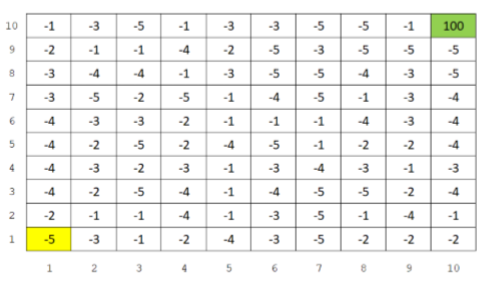
\includegraphics{Grid World.PNG}

    \textbf{Analisis Masalah:} Masalah yang diharus diselesaikan disini
yaitu, menemukan \emph{Total Reward} terbaik yang dihasilkan selama
\emph{agent} melakukan learning yaitu berupa cara menuju \emph{Initial
State} yaitu (1,1) hingga sampai pada \emph{Goal State} yaitu (10,10).
Setiap kali, \emph{agent} selesai melakukan satu kali perjalanan, maka
akan dihitung score yang diperoleh dari tiap reward yang didapat selama
\emph{agent} melakukan \emph{action} yaitu = up, down, lef, dan right.

Sebelum membuat \emph{agent} melakukan learning, terlebih dahulu kita
harus menyediakan atau mendefinisikan \emph{environment} dari jalur yang
akan dilalui oleh \emph{agent}. Desain dari \emph{environment} akan
dijelaskan pada tahap selanjutnya.

    \subsection{2. Desain Environment}\label{desain-environment}

Desain Environment yaitu tahap dimana kita akan mengatur \emph{action}
dari \emph{agent} sehingga \emph{agent} dapat memutuskan harus bergerak
kearah mana dari \emph{action} yang diberikan. Lalu, kita juga harus
mengatur berapa nilai \emph{reward} yang diperoleh jika \emph{agent}
melakukan salah satu \emph{action}. \#\#\#\# Mengatur Gerak dari Agent *
Saat aksi yang dipilih adalah 0 maka agent akan bergerak kearah atas,
artinya nilai dari koordinat y akan bertambah 1 tiap kali agent bergerak
ke atas selama belum lebih dari y = 10 * Saat aksi yang dipilih adalah 1
maka agent akan bergerak kearah bawah, artinya nilai dari koordinat y
akan berkurang 1 tiap kali agent bergerak kebawah selama belum kurang
dari y = 0 * Saat aksi yang dipilih adalah 2 maka agent akan bergerak
kearah kanan, artinya nilai dari koordinat x akan bertambah 1 tiap kali
agent bergerak selama belum lebih dari x = 10 * Saat aksi yang dipilih
adalah 3 maka agent akan bergerak kearah atas, artinya nilai dari
koordinat x akan berkurang 1 tiap kali agent bergerak selama belum
kurang dari x = 0

\paragraph{Mengisi Nilai Reward dari tiap Aksi yang
dilakukan}\label{mengisi-nilai-reward-dari-tiap-aksi-yang-dilakukan}

\begin{itemize}
\tightlist
\item
  Saat aksi yang dipilih adalah 0 maka agent akan bergerak kearah atas,
  maka reward yang diperoleh adalah saat agent berada pada koordinat y
  \textgreater{} 0 dan nilai y akan ditambahkan 1 tiap kali agent
  bergerak selama belum lebih dari y = 10 dan nilai x tetap
\item
  Saat aksi yang dipilih adalah 1 maka agent akan bergerak kearah
  bawah,maka reward yang diperoleh adalah saat agent berada pada
  koordinat y \textless{} 10 dan nilai y akan dikurangkan 1 tiap kali
  agent bergerak selama belum kurang dari y = 0 dan nilai x tetap
\item
  Saat aksi yang dipilih adalah 2 maka agent akan bergerak kearah kanan,
  maka reward yang diperoleh adalah saat agent berada pada koordinat x
  \textless{} 10 dan nilai x akan ditambahkan 1 tiap kali agent bergerak
  selama belum lebih dari x = 10 dan nilai y tetap
\item
  Saat aksi yang dipilih adalah 3 maka agent akan bergerak kearah atas,
  maka reward yang diperoleh adalah saat agent berada pada koordinat x
  \textgreater{} 0 dan nilai x akan dikurangkan 1 tiap kali agent
  bergerak selama belum kurang dari x = 0 dan nilai y tetap
\end{itemize}

    \#\#

B. LANGKAH - LANGKAH PENYELESAIAN Q-LEARNING

    \subsection{1. Import Library}\label{import-library}

    \begin{Verbatim}[commandchars=\\\{\}]
{\color{incolor}In [{\color{incolor}1}]:} \PY{k+kn}{import} \PY{n+nn}{numpy} \PY{k}{as} \PY{n+nn}{np}
        \PY{k+kn}{import} \PY{n+nn}{random}
\end{Verbatim}


    \subsection{2. Membuat Fungsi Utama untuk Update Q-table dengan Bellman
Equation}\label{membuat-fungsi-utama-untuk-update-q-table-dengan-bellman-equation}

    \begin{Verbatim}[commandchars=\\\{\}]
{\color{incolor}In [{\color{incolor}2}]:} \PY{k}{def} \PY{n+nf}{bellman}\PY{p}{(}\PY{n}{loc}\PY{p}{,}\PY{n}{dec}\PY{p}{,}\PY{n}{gamma}\PY{p}{,}\PY{n}{q}\PY{p}{)}\PY{p}{:}
            \PY{n}{a} \PY{o}{=} \PY{p}{(}\PY{n}{loc}\PY{p}{[}\PY{l+m+mi}{0}\PY{p}{]}\PY{p}{,}\PY{n}{loc}\PY{p}{[}\PY{l+m+mi}{1}\PY{p}{]}\PY{p}{)}
            \PY{n}{hasil1} \PY{o}{=} \PY{n}{reward\PYZus{}table}\PY{p}{[}\PY{n}{a}\PY{p}{]}\PY{p}{[}\PY{n}{dec}\PY{p}{]} 
            \PY{n}{d0} \PY{o}{=} \PY{n}{q}\PY{p}{[}\PY{p}{(}\PY{n}{loc}\PY{p}{[}\PY{l+m+mi}{0}\PY{p}{]}\PY{p}{,}\PY{n}{loc}\PY{p}{[}\PY{l+m+mi}{1}\PY{p}{]}\PY{p}{)}\PY{p}{]}\PY{p}{[}\PY{l+m+mi}{0}\PY{p}{]}
            \PY{n}{d1} \PY{o}{=} \PY{n}{q}\PY{p}{[}\PY{p}{(}\PY{n}{loc}\PY{p}{[}\PY{l+m+mi}{0}\PY{p}{]}\PY{p}{,}\PY{n}{loc}\PY{p}{[}\PY{l+m+mi}{1}\PY{p}{]}\PY{p}{)}\PY{p}{]}\PY{p}{[}\PY{l+m+mi}{1}\PY{p}{]}
            \PY{n}{d2} \PY{o}{=} \PY{n}{q}\PY{p}{[}\PY{p}{(}\PY{n}{loc}\PY{p}{[}\PY{l+m+mi}{0}\PY{p}{]}\PY{p}{,}\PY{n}{loc}\PY{p}{[}\PY{l+m+mi}{1}\PY{p}{]}\PY{p}{)}\PY{p}{]}\PY{p}{[}\PY{l+m+mi}{2}\PY{p}{]}
            \PY{n}{d3} \PY{o}{=} \PY{n}{q}\PY{p}{[}\PY{p}{(}\PY{n}{loc}\PY{p}{[}\PY{l+m+mi}{0}\PY{p}{]}\PY{p}{,}\PY{n}{loc}\PY{p}{[}\PY{l+m+mi}{1}\PY{p}{]}\PY{p}{)}\PY{p}{]}\PY{p}{[}\PY{l+m+mi}{3}\PY{p}{]}
            \PY{n}{hasil2} \PY{o}{=} \PY{n+nb}{max}\PY{p}{(}\PY{n}{d0}\PY{p}{,} \PY{n}{d1}\PY{p}{,} \PY{n}{d2}\PY{p}{,} \PY{n}{d3}\PY{p}{)}
            \PY{n}{hasil} \PY{o}{=} \PY{n}{hasil1} \PY{o}{+} \PY{p}{(}\PY{n}{gamma} \PY{o}{*} \PY{n}{hasil2}\PY{p}{)}
            \PY{k}{return} \PY{n}{hasil}
\end{Verbatim}


    \subsection{3. Mengatur Action dari
Agent}\label{mengatur-action-dari-agent}

    \begin{Verbatim}[commandchars=\\\{\}]
{\color{incolor}In [{\color{incolor}3}]:} \PY{k}{def} \PY{n+nf}{move}\PY{p}{(}\PY{n}{loc}\PY{p}{,}\PY{n}{dec}\PY{p}{)}\PY{p}{:}
            \PY{k}{if} \PY{n}{dec} \PY{o}{==} \PY{l+m+mi}{0} \PY{p}{:}
                \PY{k}{if} \PY{n}{loc}\PY{p}{[}\PY{l+m+mi}{1}\PY{p}{]} \PY{o}{\PYZgt{}} \PY{l+m+mi}{0} \PY{p}{:}
                    \PY{n}{loc}\PY{p}{[}\PY{l+m+mi}{1}\PY{p}{]} \PY{o}{=} \PY{n}{loc}\PY{p}{[}\PY{l+m+mi}{1}\PY{p}{]} \PY{o}{\PYZhy{}} \PY{l+m+mi}{1}
            \PY{k}{elif} \PY{n}{dec} \PY{o}{==} \PY{l+m+mi}{1} \PY{p}{:}
                \PY{k}{if} \PY{n}{loc}\PY{p}{[}\PY{l+m+mi}{1}\PY{p}{]} \PY{o}{\PYZlt{}} \PY{l+m+mi}{9} \PY{p}{:}
                    \PY{n}{loc}\PY{p}{[}\PY{l+m+mi}{1}\PY{p}{]} \PY{o}{=} \PY{n}{loc}\PY{p}{[}\PY{l+m+mi}{1}\PY{p}{]} \PY{o}{+} \PY{l+m+mi}{1}
            \PY{k}{elif} \PY{n}{dec} \PY{o}{==} \PY{l+m+mi}{2} \PY{p}{:}
                \PY{k}{if} \PY{n}{loc}\PY{p}{[}\PY{l+m+mi}{0}\PY{p}{]} \PY{o}{\PYZlt{}} \PY{l+m+mi}{9} \PY{p}{:}
                    \PY{n}{loc}\PY{p}{[}\PY{l+m+mi}{0}\PY{p}{]} \PY{o}{=} \PY{n}{loc}\PY{p}{[}\PY{l+m+mi}{0}\PY{p}{]} \PY{o}{+} \PY{l+m+mi}{1}
            \PY{k}{elif} \PY{n}{dec} \PY{o}{==} \PY{l+m+mi}{3} \PY{p}{:}
                \PY{k}{if} \PY{n}{loc}\PY{p}{[}\PY{l+m+mi}{0}\PY{p}{]} \PY{o}{\PYZgt{}} \PY{l+m+mi}{0} \PY{p}{:}
                    \PY{n}{loc}\PY{p}{[}\PY{l+m+mi}{0}\PY{p}{]} \PY{o}{=} \PY{n}{loc}\PY{p}{[}\PY{l+m+mi}{0}\PY{p}{]} \PY{o}{\PYZhy{}} \PY{l+m+mi}{1}
\end{Verbatim}


    \subsection{4. Mengatur Nilai Reward dari Tiap
Decision}\label{mengatur-nilai-reward-dari-tiap-decision}

    \begin{Verbatim}[commandchars=\\\{\}]
{\color{incolor}In [{\color{incolor}4}]:} \PY{k}{def} \PY{n+nf}{r\PYZus{}up}\PY{p}{(}\PY{n}{loc}\PY{p}{)}\PY{p}{:}
            \PY{k}{global} \PY{n}{reward}
            \PY{k}{if} \PY{n}{loc}\PY{p}{[}\PY{l+m+mi}{1}\PY{p}{]} \PY{o}{\PYZgt{}} \PY{l+m+mi}{0} \PY{p}{:}
                \PY{n}{y} \PY{o}{=} \PY{n}{loc}\PY{p}{[}\PY{l+m+mi}{1}\PY{p}{]} \PY{o}{\PYZhy{}} \PY{l+m+mi}{1}
            \PY{k}{else} \PY{p}{:}
                \PY{k}{return} \PY{l+m+mi}{0}
            \PY{k}{return} \PY{n}{reward}\PY{p}{[}\PY{n}{loc}\PY{p}{[}\PY{l+m+mi}{0}\PY{p}{]}\PY{p}{]}\PY{p}{[}\PY{n}{y}\PY{p}{]}
        
        \PY{k}{def} \PY{n+nf}{r\PYZus{}down}\PY{p}{(}\PY{n}{loc}\PY{p}{)}\PY{p}{:}
            \PY{k}{global} \PY{n}{reward}
            \PY{k}{if} \PY{n}{loc}\PY{p}{[}\PY{l+m+mi}{1}\PY{p}{]} \PY{o}{\PYZlt{}} \PY{l+m+mi}{9} \PY{p}{:}
                \PY{n}{y} \PY{o}{=} \PY{n}{loc}\PY{p}{[}\PY{l+m+mi}{1}\PY{p}{]} \PY{o}{+} \PY{l+m+mi}{1}
            \PY{k}{else} \PY{p}{:}
                \PY{k}{return} \PY{l+m+mi}{0}
            \PY{k}{return} \PY{n}{reward}\PY{p}{[}\PY{n}{loc}\PY{p}{[}\PY{l+m+mi}{0}\PY{p}{]}\PY{p}{]}\PY{p}{[}\PY{n}{y}\PY{p}{]}
        
        \PY{k}{def} \PY{n+nf}{r\PYZus{}right}\PY{p}{(}\PY{n}{loc}\PY{p}{)}\PY{p}{:}
            \PY{k}{global} \PY{n}{reward}
            \PY{k}{if} \PY{n}{loc}\PY{p}{[}\PY{l+m+mi}{0}\PY{p}{]} \PY{o}{\PYZlt{}} \PY{l+m+mi}{9} \PY{p}{:}
                \PY{n}{x} \PY{o}{=} \PY{n}{loc}\PY{p}{[}\PY{l+m+mi}{0}\PY{p}{]} \PY{o}{+} \PY{l+m+mi}{1}
            \PY{k}{else} \PY{p}{:}
                \PY{k}{return} \PY{l+m+mi}{0}
            \PY{k}{return} \PY{n}{reward}\PY{p}{[}\PY{n}{x}\PY{p}{]}\PY{p}{[}\PY{n}{loc}\PY{p}{[}\PY{l+m+mi}{1}\PY{p}{]}\PY{p}{]}
        
        \PY{k}{def} \PY{n+nf}{r\PYZus{}left}\PY{p}{(}\PY{n}{loc}\PY{p}{)}\PY{p}{:}
            \PY{k}{global} \PY{n}{reward}
            \PY{k}{if} \PY{n}{loc}\PY{p}{[}\PY{l+m+mi}{0}\PY{p}{]} \PY{o}{\PYZgt{}} \PY{l+m+mi}{0} \PY{p}{:}
                \PY{n}{x} \PY{o}{=} \PY{n}{loc}\PY{p}{[}\PY{l+m+mi}{0}\PY{p}{]} \PY{o}{\PYZhy{}} \PY{l+m+mi}{1}
            \PY{k}{else} \PY{p}{:}
                \PY{k}{return} \PY{l+m+mi}{0}
            \PY{k}{return} \PY{n}{reward}\PY{p}{[}\PY{n}{x}\PY{p}{]}\PY{p}{[}\PY{n}{loc}\PY{p}{[}\PY{l+m+mi}{1}\PY{p}{]}\PY{p}{]}
\end{Verbatim}


    \subsection{5. Mempersiapkan Tiap Variable yang Dibutuhkan dan Loading
Data
File}\label{mempersiapkan-tiap-variable-yang-dibutuhkan-dan-loading-data-file}

    \begin{Verbatim}[commandchars=\\\{\}]
{\color{incolor}In [{\color{incolor}5}]:} \PY{n}{start} \PY{o}{=} \PY{p}{[}\PY{l+m+mi}{9}\PY{p}{,}\PY{l+m+mi}{0}\PY{p}{]}
        \PY{n}{x} \PY{o}{=} \PY{l+m+mi}{10}
        \PY{n}{y} \PY{o}{=} \PY{l+m+mi}{10}
        \PY{n}{finish} \PY{o}{=} \PY{p}{[}\PY{l+m+mi}{0}\PY{p}{,}\PY{l+m+mi}{9}\PY{p}{]}
        \PY{n}{initial} \PY{o}{=} \PY{p}{[}\PY{l+m+mi}{0}\PY{p}{,}\PY{l+m+mi}{0}\PY{p}{,}\PY{l+m+mi}{0}\PY{p}{,}\PY{l+m+mi}{0}\PY{p}{]}
        \PY{n}{q\PYZus{}table} \PY{o}{=} \PY{p}{\PYZob{}}\PY{p}{\PYZcb{}}
        \PY{n}{reward} \PY{o}{=} \PY{n}{np}\PY{o}{.}\PY{n}{loadtxt}\PY{p}{(}\PY{l+s+s2}{\PYZdq{}}\PY{l+s+s2}{DataTugasML3.txt}\PY{l+s+s2}{\PYZdq{}}\PY{p}{)}
        \PY{n}{states} \PY{o}{=} \PY{p}{[}\PY{p}{]}
        \PY{n}{reward\PYZus{}table} \PY{o}{=} \PY{p}{\PYZob{}}\PY{p}{\PYZcb{}}
        \PY{n}{maks} \PY{o}{=} \PY{o}{\PYZhy{}}\PY{l+m+mi}{99999}
        \PY{n}{gamma} \PY{o}{=} \PY{l+m+mf}{0.5}
        
        \PY{n+nb}{print}\PY{p}{(}\PY{n}{reward}\PY{p}{)}
\end{Verbatim}


    \begin{Verbatim}[commandchars=\\\{\}]
[[ -1.  -3.  -5.  -1.  -3.  -3.  -5.  -5.  -1. 100.]
 [ -2.  -1.  -1.  -4.  -2.  -5.  -3.  -5.  -5.  -5.]
 [ -3.  -4.  -4.  -1.  -3.  -5.  -5.  -4.  -3.  -5.]
 [ -3.  -5.  -2.  -5.  -1.  -4.  -5.  -1.  -3.  -4.]
 [ -4.  -3.  -3.  -2.  -1.  -1.  -1.  -4.  -3.  -4.]
 [ -4.  -2.  -5.  -2.  -4.  -5.  -1.  -2.  -2.  -4.]
 [ -4.  -3.  -2.  -3.  -1.  -3.  -4.  -3.  -1.  -3.]
 [ -4.  -2.  -5.  -4.  -1.  -4.  -5.  -5.  -2.  -4.]
 [ -2.  -1.  -1.  -4.  -1.  -3.  -5.  -1.  -4.  -1.]
 [ -5.  -3.  -1.  -2.  -4.  -3.  -5.  -2.  -2.  -2.]]

    \end{Verbatim}

    \subsection{6. Menginputkan Koordinat X dan Y sebagai
State}\label{menginputkan-koordinat-x-dan-y-sebagai-state}

    \begin{Verbatim}[commandchars=\\\{\}]
{\color{incolor}In [{\color{incolor}6}]:} \PY{k}{for} \PY{n}{i} \PY{o+ow}{in} \PY{n+nb}{range}\PY{p}{(}\PY{n}{x}\PY{p}{)}\PY{p}{:}
            \PY{k}{for} \PY{n}{j} \PY{o+ow}{in} \PY{n+nb}{range}\PY{p}{(}\PY{n}{y}\PY{p}{)}\PY{p}{:}
                \PY{n}{states}\PY{o}{.}\PY{n}{append}\PY{p}{(}\PY{p}{(}\PY{n}{i}\PY{p}{,}\PY{n}{j}\PY{p}{)}\PY{p}{)}
\end{Verbatim}


    \subsection{7. Membuat Reward Table berukuran 100 x
4}\label{membuat-reward-table-berukuran-100-x-4}

    \begin{Verbatim}[commandchars=\\\{\}]
{\color{incolor}In [{\color{incolor}7}]:} \PY{k}{for} \PY{n}{i} \PY{o+ow}{in} \PY{n+nb}{range}\PY{p}{(}\PY{n}{x}\PY{o}{*}\PY{n}{y}\PY{p}{)} \PY{p}{:}
            \PY{n}{reward\PYZus{}table}\PY{p}{[}\PY{n}{states}\PY{p}{[}\PY{n}{i}\PY{p}{]}\PY{p}{]} \PY{o}{=} \PY{n}{initial}
        \PY{n+nb}{print}\PY{p}{(}\PY{n}{reward\PYZus{}table}\PY{p}{)}
\end{Verbatim}


    \begin{Verbatim}[commandchars=\\\{\}]
\{(0, 0): [0, 0, 0, 0], (0, 1): [0, 0, 0, 0], (0, 2): [0, 0, 0, 0], (0, 3): [0, 0, 0, 0], (0, 4): [0, 0, 0, 0], (0, 5): [0, 0, 0, 0], (0, 6): [0, 0, 0, 0], (0, 7): [0, 0, 0, 0], (0, 8): [0, 0, 0, 0], (0, 9): [0, 0, 0, 0], (1, 0): [0, 0, 0, 0], (1, 1): [0, 0, 0, 0], (1, 2): [0, 0, 0, 0], (1, 3): [0, 0, 0, 0], (1, 4): [0, 0, 0, 0], (1, 5): [0, 0, 0, 0], (1, 6): [0, 0, 0, 0], (1, 7): [0, 0, 0, 0], (1, 8): [0, 0, 0, 0], (1, 9): [0, 0, 0, 0], (2, 0): [0, 0, 0, 0], (2, 1): [0, 0, 0, 0], (2, 2): [0, 0, 0, 0], (2, 3): [0, 0, 0, 0], (2, 4): [0, 0, 0, 0], (2, 5): [0, 0, 0, 0], (2, 6): [0, 0, 0, 0], (2, 7): [0, 0, 0, 0], (2, 8): [0, 0, 0, 0], (2, 9): [0, 0, 0, 0], (3, 0): [0, 0, 0, 0], (3, 1): [0, 0, 0, 0], (3, 2): [0, 0, 0, 0], (3, 3): [0, 0, 0, 0], (3, 4): [0, 0, 0, 0], (3, 5): [0, 0, 0, 0], (3, 6): [0, 0, 0, 0], (3, 7): [0, 0, 0, 0], (3, 8): [0, 0, 0, 0], (3, 9): [0, 0, 0, 0], (4, 0): [0, 0, 0, 0], (4, 1): [0, 0, 0, 0], (4, 2): [0, 0, 0, 0], (4, 3): [0, 0, 0, 0], (4, 4): [0, 0, 0, 0], (4, 5): [0, 0, 0, 0], (4, 6): [0, 0, 0, 0], (4, 7): [0, 0, 0, 0], (4, 8): [0, 0, 0, 0], (4, 9): [0, 0, 0, 0], (5, 0): [0, 0, 0, 0], (5, 1): [0, 0, 0, 0], (5, 2): [0, 0, 0, 0], (5, 3): [0, 0, 0, 0], (5, 4): [0, 0, 0, 0], (5, 5): [0, 0, 0, 0], (5, 6): [0, 0, 0, 0], (5, 7): [0, 0, 0, 0], (5, 8): [0, 0, 0, 0], (5, 9): [0, 0, 0, 0], (6, 0): [0, 0, 0, 0], (6, 1): [0, 0, 0, 0], (6, 2): [0, 0, 0, 0], (6, 3): [0, 0, 0, 0], (6, 4): [0, 0, 0, 0], (6, 5): [0, 0, 0, 0], (6, 6): [0, 0, 0, 0], (6, 7): [0, 0, 0, 0], (6, 8): [0, 0, 0, 0], (6, 9): [0, 0, 0, 0], (7, 0): [0, 0, 0, 0], (7, 1): [0, 0, 0, 0], (7, 2): [0, 0, 0, 0], (7, 3): [0, 0, 0, 0], (7, 4): [0, 0, 0, 0], (7, 5): [0, 0, 0, 0], (7, 6): [0, 0, 0, 0], (7, 7): [0, 0, 0, 0], (7, 8): [0, 0, 0, 0], (7, 9): [0, 0, 0, 0], (8, 0): [0, 0, 0, 0], (8, 1): [0, 0, 0, 0], (8, 2): [0, 0, 0, 0], (8, 3): [0, 0, 0, 0], (8, 4): [0, 0, 0, 0], (8, 5): [0, 0, 0, 0], (8, 6): [0, 0, 0, 0], (8, 7): [0, 0, 0, 0], (8, 8): [0, 0, 0, 0], (8, 9): [0, 0, 0, 0], (9, 0): [0, 0, 0, 0], (9, 1): [0, 0, 0, 0], (9, 2): [0, 0, 0, 0], (9, 3): [0, 0, 0, 0], (9, 4): [0, 0, 0, 0], (9, 5): [0, 0, 0, 0], (9, 6): [0, 0, 0, 0], (9, 7): [0, 0, 0, 0], (9, 8): [0, 0, 0, 0], (9, 9): [0, 0, 0, 0]\}

    \end{Verbatim}

    \subsection{8. Membangun Environtment pada Reward
Table}\label{membangun-environtment-pada-reward-table}

    \begin{Verbatim}[commandchars=\\\{\}]
{\color{incolor}In [{\color{incolor}8}]:} \PY{k}{for} \PY{n}{dec} \PY{o+ow}{in} \PY{n+nb}{range}\PY{p}{(}\PY{l+m+mi}{0}\PY{p}{,}\PY{l+m+mi}{4}\PY{p}{)}\PY{p}{:}
            \PY{k}{for} \PY{n}{i} \PY{o+ow}{in} \PY{n+nb}{range}\PY{p}{(}\PY{n+nb}{len}\PY{p}{(}\PY{n}{reward}\PY{p}{)}\PY{p}{)}\PY{p}{:}
                \PY{k}{for} \PY{n}{j} \PY{o+ow}{in} \PY{n+nb}{range}\PY{p}{(}\PY{n+nb}{len}\PY{p}{(}\PY{n}{reward}\PY{p}{[}\PY{l+m+mi}{0}\PY{p}{]}\PY{p}{)}\PY{p}{)}\PY{p}{:}
                    \PY{n}{loc} \PY{o}{=} \PY{p}{[}\PY{n}{i}\PY{p}{,}\PY{n}{j}\PY{p}{]}
                    \PY{n}{temp} \PY{o}{=} \PY{p}{[}\PY{p}{]}
                    \PY{n}{temp}\PY{o}{.}\PY{n}{clear}
                    \PY{n}{temp}\PY{o}{.}\PY{n}{append}\PY{p}{(}\PY{n}{r\PYZus{}up}\PY{p}{(}\PY{n}{loc}\PY{p}{)}\PY{p}{)}
                    \PY{n}{temp}\PY{o}{.}\PY{n}{append}\PY{p}{(}\PY{n}{r\PYZus{}down}\PY{p}{(}\PY{n}{loc}\PY{p}{)}\PY{p}{)}
                    \PY{n}{temp}\PY{o}{.}\PY{n}{append}\PY{p}{(}\PY{n}{r\PYZus{}right}\PY{p}{(}\PY{n}{loc}\PY{p}{)}\PY{p}{)}
                    \PY{n}{temp}\PY{o}{.}\PY{n}{append}\PY{p}{(}\PY{n}{r\PYZus{}left}\PY{p}{(}\PY{n}{loc}\PY{p}{)}\PY{p}{)}
                    \PY{n}{reward\PYZus{}table}\PY{p}{[}\PY{p}{(}\PY{n}{i}\PY{p}{,}\PY{n}{j}\PY{p}{)}\PY{p}{]} \PY{o}{=} \PY{n}{temp}
\end{Verbatim}


    \subsection{9. Membuat Q Table dengan Value Seluruhnya adalah 0
berukuran 100 x
4}\label{membuat-q-table-dengan-value-seluruhnya-adalah-0-berukuran-100-x-4}

    \begin{Verbatim}[commandchars=\\\{\}]
{\color{incolor}In [{\color{incolor}9}]:} \PY{k}{for} \PY{n}{i} \PY{o+ow}{in} \PY{n+nb}{range}\PY{p}{(}\PY{n}{x}\PY{o}{*}\PY{n}{y}\PY{p}{)} \PY{p}{:}
            \PY{n}{q\PYZus{}table}\PY{p}{[}\PY{n}{states}\PY{p}{[}\PY{n}{i}\PY{p}{]}\PY{p}{]} \PY{o}{=} \PY{n}{initial}
        \PY{n+nb}{print}\PY{p}{(}\PY{n}{q\PYZus{}table}\PY{p}{)}
\end{Verbatim}


    \begin{Verbatim}[commandchars=\\\{\}]
\{(0, 0): [0, 0, 0, 0], (0, 1): [0, 0, 0, 0], (0, 2): [0, 0, 0, 0], (0, 3): [0, 0, 0, 0], (0, 4): [0, 0, 0, 0], (0, 5): [0, 0, 0, 0], (0, 6): [0, 0, 0, 0], (0, 7): [0, 0, 0, 0], (0, 8): [0, 0, 0, 0], (0, 9): [0, 0, 0, 0], (1, 0): [0, 0, 0, 0], (1, 1): [0, 0, 0, 0], (1, 2): [0, 0, 0, 0], (1, 3): [0, 0, 0, 0], (1, 4): [0, 0, 0, 0], (1, 5): [0, 0, 0, 0], (1, 6): [0, 0, 0, 0], (1, 7): [0, 0, 0, 0], (1, 8): [0, 0, 0, 0], (1, 9): [0, 0, 0, 0], (2, 0): [0, 0, 0, 0], (2, 1): [0, 0, 0, 0], (2, 2): [0, 0, 0, 0], (2, 3): [0, 0, 0, 0], (2, 4): [0, 0, 0, 0], (2, 5): [0, 0, 0, 0], (2, 6): [0, 0, 0, 0], (2, 7): [0, 0, 0, 0], (2, 8): [0, 0, 0, 0], (2, 9): [0, 0, 0, 0], (3, 0): [0, 0, 0, 0], (3, 1): [0, 0, 0, 0], (3, 2): [0, 0, 0, 0], (3, 3): [0, 0, 0, 0], (3, 4): [0, 0, 0, 0], (3, 5): [0, 0, 0, 0], (3, 6): [0, 0, 0, 0], (3, 7): [0, 0, 0, 0], (3, 8): [0, 0, 0, 0], (3, 9): [0, 0, 0, 0], (4, 0): [0, 0, 0, 0], (4, 1): [0, 0, 0, 0], (4, 2): [0, 0, 0, 0], (4, 3): [0, 0, 0, 0], (4, 4): [0, 0, 0, 0], (4, 5): [0, 0, 0, 0], (4, 6): [0, 0, 0, 0], (4, 7): [0, 0, 0, 0], (4, 8): [0, 0, 0, 0], (4, 9): [0, 0, 0, 0], (5, 0): [0, 0, 0, 0], (5, 1): [0, 0, 0, 0], (5, 2): [0, 0, 0, 0], (5, 3): [0, 0, 0, 0], (5, 4): [0, 0, 0, 0], (5, 5): [0, 0, 0, 0], (5, 6): [0, 0, 0, 0], (5, 7): [0, 0, 0, 0], (5, 8): [0, 0, 0, 0], (5, 9): [0, 0, 0, 0], (6, 0): [0, 0, 0, 0], (6, 1): [0, 0, 0, 0], (6, 2): [0, 0, 0, 0], (6, 3): [0, 0, 0, 0], (6, 4): [0, 0, 0, 0], (6, 5): [0, 0, 0, 0], (6, 6): [0, 0, 0, 0], (6, 7): [0, 0, 0, 0], (6, 8): [0, 0, 0, 0], (6, 9): [0, 0, 0, 0], (7, 0): [0, 0, 0, 0], (7, 1): [0, 0, 0, 0], (7, 2): [0, 0, 0, 0], (7, 3): [0, 0, 0, 0], (7, 4): [0, 0, 0, 0], (7, 5): [0, 0, 0, 0], (7, 6): [0, 0, 0, 0], (7, 7): [0, 0, 0, 0], (7, 8): [0, 0, 0, 0], (7, 9): [0, 0, 0, 0], (8, 0): [0, 0, 0, 0], (8, 1): [0, 0, 0, 0], (8, 2): [0, 0, 0, 0], (8, 3): [0, 0, 0, 0], (8, 4): [0, 0, 0, 0], (8, 5): [0, 0, 0, 0], (8, 6): [0, 0, 0, 0], (8, 7): [0, 0, 0, 0], (8, 8): [0, 0, 0, 0], (8, 9): [0, 0, 0, 0], (9, 0): [0, 0, 0, 0], (9, 1): [0, 0, 0, 0], (9, 2): [0, 0, 0, 0], (9, 3): [0, 0, 0, 0], (9, 4): [0, 0, 0, 0], (9, 5): [0, 0, 0, 0], (9, 6): [0, 0, 0, 0], (9, 7): [0, 0, 0, 0], (9, 8): [0, 0, 0, 0], (9, 9): [0, 0, 0, 0]\}

    \end{Verbatim}

    \section{10. Q Learning}\label{q-learning}

    \begin{Verbatim}[commandchars=\\\{\}]
{\color{incolor}In [{\color{incolor}11}]:} \PY{k}{for} \PY{n}{i} \PY{o+ow}{in} \PY{n+nb}{range}\PY{p}{(}\PY{l+m+mi}{0}\PY{p}{,}\PY{l+m+mi}{100}\PY{p}{)}\PY{p}{:}
             \PY{n}{score} \PY{o}{=} \PY{l+m+mi}{0}
             \PY{n}{q} \PY{o}{=} \PY{n}{q\PYZus{}table}
             \PY{n}{end} \PY{o}{=} \PY{k+kc}{False}
             \PY{n}{loc} \PY{o}{=} \PY{p}{[}\PY{l+m+mi}{9}\PY{p}{,}\PY{l+m+mi}{0}\PY{p}{]}
             \PY{k}{while} \PY{n}{end} \PY{o}{==} \PY{k+kc}{False}\PY{p}{:}
                 \PY{c+c1}{\PYZsh{} up = 0 , down = 1 , right = 2 ,left = 3}
                 \PY{n}{dec} \PY{o}{=} \PY{n}{random}\PY{o}{.}\PY{n}{randint}\PY{p}{(}\PY{l+m+mi}{0}\PY{p}{,}\PY{l+m+mi}{3}\PY{p}{)}
                 \PY{n}{bell} \PY{o}{=} \PY{n}{bellman}\PY{p}{(}\PY{n}{loc}\PY{p}{,}\PY{n}{dec}\PY{p}{,}\PY{n}{gamma}\PY{p}{,}\PY{n}{q}\PY{p}{)}
                 \PY{n}{q}\PY{p}{[}\PY{p}{(}\PY{n}{loc}\PY{p}{[}\PY{l+m+mi}{0}\PY{p}{]}\PY{p}{,}\PY{n}{loc}\PY{p}{[}\PY{l+m+mi}{1}\PY{p}{]}\PY{p}{)}\PY{p}{]}\PY{p}{[}\PY{n}{dec}\PY{p}{]} \PY{o}{=} \PY{n}{bell}
                 \PY{k}{if} \PY{n}{dec} \PY{o}{==} \PY{l+m+mi}{0} \PY{p}{:} 
                     \PY{n}{move}\PY{p}{(}\PY{n}{loc}\PY{p}{,}\PY{n}{dec}\PY{p}{)}
                     \PY{n}{score} \PY{o}{=} \PY{n}{score} \PY{o}{+} \PY{n}{r\PYZus{}up}\PY{p}{(}\PY{n}{loc}\PY{p}{)}
                 \PY{k}{elif} \PY{n}{dec} \PY{o}{==} \PY{l+m+mi}{1}\PY{p}{:}
                     \PY{n}{move}\PY{p}{(}\PY{n}{loc}\PY{p}{,}\PY{n}{dec}\PY{p}{)}
                     \PY{n}{score} \PY{o}{=} \PY{n}{score} \PY{o}{+} \PY{n}{r\PYZus{}down}\PY{p}{(}\PY{n}{loc}\PY{p}{)}
                 \PY{k}{elif} \PY{n}{dec} \PY{o}{==} \PY{l+m+mi}{2}\PY{p}{:}
                     \PY{n}{move}\PY{p}{(}\PY{n}{loc}\PY{p}{,}\PY{n}{dec}\PY{p}{)}
                     \PY{n}{score} \PY{o}{=} \PY{n}{score} \PY{o}{+} \PY{n}{r\PYZus{}right}\PY{p}{(}\PY{n}{loc}\PY{p}{)}
                 \PY{k}{elif} \PY{n}{dec} \PY{o}{==} \PY{l+m+mi}{3} \PY{p}{:}
                     \PY{n}{move}\PY{p}{(}\PY{n}{loc}\PY{p}{,}\PY{n}{dec}\PY{p}{)}
                     \PY{n}{score} \PY{o}{=} \PY{n}{score} \PY{o}{+} \PY{n}{r\PYZus{}left}\PY{p}{(}\PY{n}{loc}\PY{p}{)}
         
                 \PY{k}{if} \PY{n}{loc}\PY{p}{[}\PY{l+m+mi}{0}\PY{p}{]} \PY{o}{==} \PY{n}{finish}\PY{p}{[}\PY{l+m+mi}{0}\PY{p}{]} \PY{o+ow}{and} \PY{n}{loc}\PY{p}{[}\PY{l+m+mi}{1}\PY{p}{]} \PY{o}{==} \PY{n}{finish}\PY{p}{[}\PY{l+m+mi}{1}\PY{p}{]} \PY{p}{:}
                     \PY{n}{end} \PY{o}{=} \PY{k+kc}{True}
             \PY{n+nb}{print}\PY{p}{(}\PY{l+s+s2}{\PYZdq{}}\PY{l+s+s2}{score = }\PY{l+s+s2}{\PYZdq{}}\PY{p}{,}\PY{n}{score}\PY{p}{)}
             \PY{k}{if} \PY{n}{maks} \PY{o}{\PYZlt{}} \PY{n}{score} \PY{p}{:}
                 \PY{n}{maks} \PY{o}{=} \PY{n}{score}  
             \PY{n}{q\PYZus{}table} \PY{o}{=} \PY{n}{q}
         
         \PY{n+nb}{print}\PY{p}{(}\PY{p}{)}
         \PY{n+nb}{print}\PY{p}{(}\PY{l+s+s2}{\PYZdq{}}\PY{l+s+s2}{Maximum: }\PY{l+s+s2}{\PYZdq{}}\PY{p}{,}\PY{n}{maks}\PY{p}{)}
\end{Verbatim}


    \begin{Verbatim}[commandchars=\\\{\}]
score =  -440.0
score =  -583.0
score =  -723.0
score =  -859.0
score =  -673.0
score =  -630.0
score =  -623.0
score =  -862.0
score =  -450.0
score =  -2568.0
score =  -2257.0
score =  -898.0
score =  -625.0
score =  -2530.0
score =  -1590.0
score =  -394.0
score =  -366.0
score =  -1153.0
score =  -141.0
score =  -98.0
score =  -1238.0
score =  -1036.0
score =  -1873.0
score =  -1451.0
score =  -2399.0
score =  -778.0
score =  -3658.0
score =  -4017.0
score =  -1319.0
score =  -480.0
score =  -581.0
score =  -770.0
score =  -1369.0
score =  -1961.0
score =  -502.0
score =  -695.0
score =  -190.0
score =  -1322.0
score =  -2697.0
score =  -3120.0
score =  -1469.0
score =  -2790.0
score =  -3038.0
score =  -187.0
score =  -775.0
score =  -2487.0
score =  -1050.0
score =  -1238.0
score =  -3356.0
score =  -13.0
score =  -2749.0
score =  -1229.0
score =  -639.0
score =  -331.0
score =  -5560.0
score =  -1502.0
score =  -2262.0
score =  -2988.0
score =  -1662.0
score =  -635.0
score =  -2873.0
score =  -806.0
score =  -647.0
score =  -484.0
score =  -14.0
score =  -918.0
score =  -845.0
score =  -1835.0
score =  -6859.0
score =  -570.0
score =  -811.0
score =  -90.0
score =  -473.0
score =  48.0
score =  -2257.0
score =  -96.0
score =  -974.0
score =  -394.0
score =  -803.0
score =  -3138.0
score =  -1441.0
score =  -1569.0
score =  -3419.0
score =  -562.0
score =  -5137.0
score =  -1973.0
score =  -841.0
score =  -216.0
score =  -1829.0
score =  -331.0
score =  -362.0
score =  -148.0
score =  -1374.0
score =  -228.0
score =  -1977.0
score =  -491.0
score =  -873.0
score =  -1484.0
score =  -1805.0
score =  -275.0

Maximum:  48.0

    \end{Verbatim}

    \#

C. HASIL EKSPERIMEN

    Hasil eksperimen yang diperoleh adalah nilai total reward paling bagus
selama melakukan eksperimen Q-Learning pada \emph{agent} adalah 48.0
dengan percobaan melakukan episode sebanyak 100 kali episode. Hal ini
menyatakan bahwa, \emph{agent} dengan 100 kali episode belum cukup baik
memahami environment yang dibuat.

Hal ini terjadi dikarenakan beberapa kemungkinan yang saya lakukan pada
pemrograman. Beberapa hal tersebut saya perkirakan adalah: 1. Aksi yang
akan dilakukan diputuskan secara random (dapat dilihat pada bagian 10.
Q-Learning) 2. Pada saat perhitungan score dengan reward yang diperoleh
(dapat dilihat pada bagian 10. Q-Learning) 3. Pada penentuan reward pada
reward table sebagai environment yang harus dipelajari oleh \emph{agent}
(dapat dilihat pada bagian 8. Membangun environment pada reward table)


    % Add a bibliography block to the postdoc
    
    
    
    \end{document}
